%%%%%%%%%%%%%%%%%%%%%%%%%%%%%%%%%%%%%%%%%%%%%%%%%%%%%%%%%%%%%%%%%%%%%%%%%%%
%
% Template for a LaTex article in English.
%
%%%%%%%%%%%%%%%%%%%%%%%%%%%%%%%%%%%%%%%%%%%%%%%%%%%%%%%%%%%%%%%%%%%%%%%%%%%

\documentclass{article}

% AMS packages:
\usepackage{amsmath, amsthm, amsfonts}
\usepackage{algorithm}
\usepackage[hyperref, UTF8]{ctex}
\usepackage[noend]{algpseudocode}
\usepackage{graphicx}
\graphicspath{ {images/} }

% Theorems
%-----------------------------------------------------------------
\newtheorem{thm}{Theorem}[section]
\newtheorem{cor}[thm]{Corollary}
\newtheorem{lem}[thm]{Lemma}
\newtheorem{prop}[thm]{Proposition}
\theoremstyle{definition}
\newtheorem{defn}[thm]{Definition}
\theoremstyle{remark}
\newtheorem{rem}[thm]{Remark}

\makeatletter
\def\BState{\State\hskip-\ALG@thistlm}
\makeatother
%\newcommand*{\rom}[1]{\expandafter\@slowromancap\romannumeral #1@}
\newcommand{\rom}[1]{\uppercase\expandafter{\romannumeral #1\relax}}
% Shortcuts.
% One can define new commands to shorten frequently used
% constructions. As an example, this defines the R and Z used
% for the real and integer numbers.
%-----------------------------------------------------------------
\def\RR{\mathbb{R}}
\def\ZZ{\mathbb{Z}}

% Similarly, one can define commands that take arguments. In this
% example we define a command for the absolute value.
% -----------------------------------------------------------------
\newcommand{\abs}[1]{\left\vert#1\right\vert}

% Operators
% New operators must defined as such to have them typeset
% correctly. As an example we define the Jacobian:
% -----------------------------------------------------------------
\DeclareMathOperator{\Jac}{Jac}

%-----------------------------------------------------------------
\title{Work Report}
\author{ShengweiZHANG\\
  %% \small Dept. Templates and Editors\\
  %% \small E12345\\
  %% \small Spain
}

\begin{document}
\maketitle

%% \abstract{Compiling Embedded\_thin\_shell progress}
\section{上周工作}
\begin{itemize}
	\item 将代码移植到Windows平台上.
	\item 滤波输出结果res.obj中每个点到expected.obj中最近点的距离的可视化显示(Figure 1). 
\end{itemize}
\begin{equation}
	dis(v_i) = ||v_i -N(v_i)||/r
\end{equation}
这里$dis(v_i)$是双边滤波结果的每个顶点与期望结果顶点值得差,$N(v_i)$是从expect模型中找到与$v_i$ 最近的点, r是input模型的包围球直径.
从可视化的角度不太满足我们的要求,因为模型变化比较剧烈的边界部分dist比较大,而相对平坦区域dist比较小. 而dist较小的平坦区域却仍有可能带有很多噪声.不知道dist的平均值能否比较合理表示两个模型的difference.
\begin{figure}[H]
	\onecolumn
	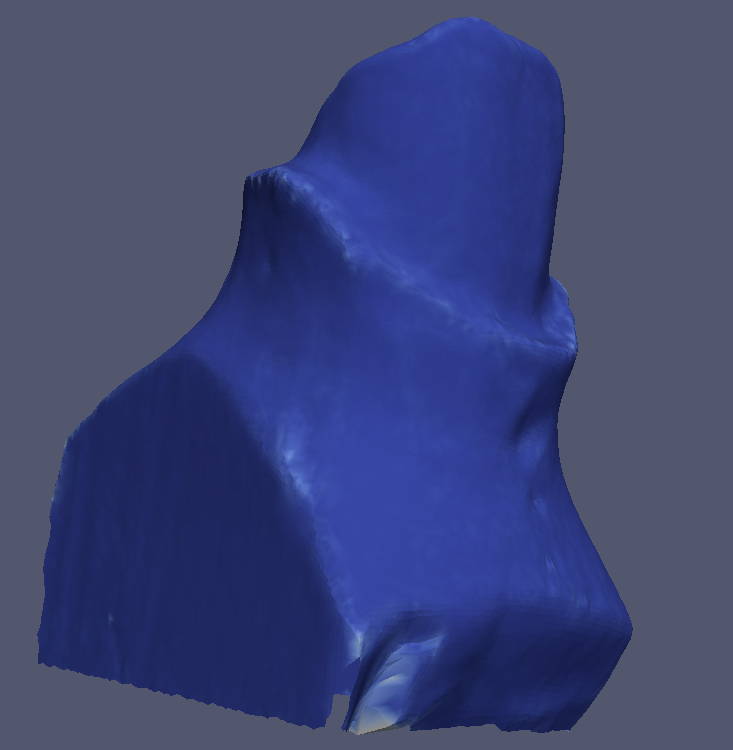
\includegraphics[width=2.3cm]{diffv}
	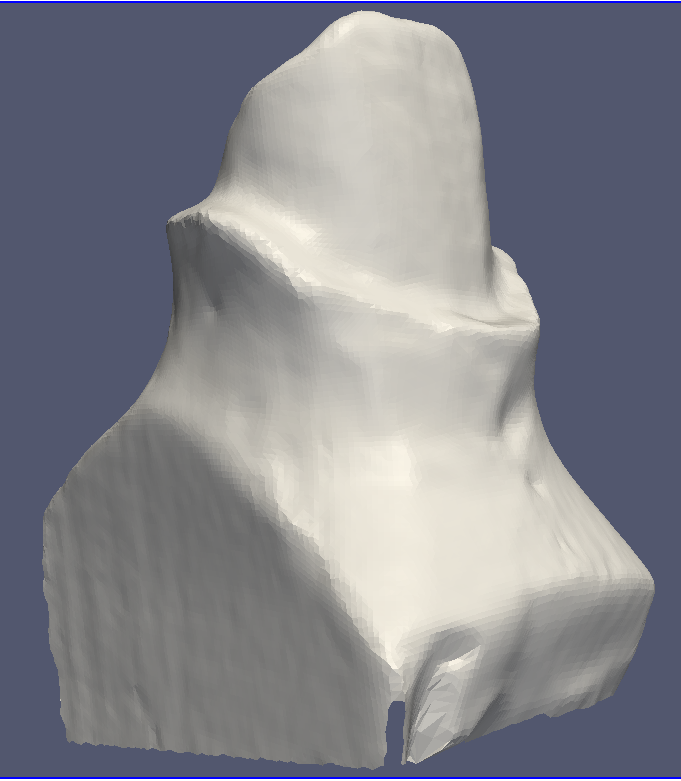
\includegraphics[width=2cm]{our_basic}
	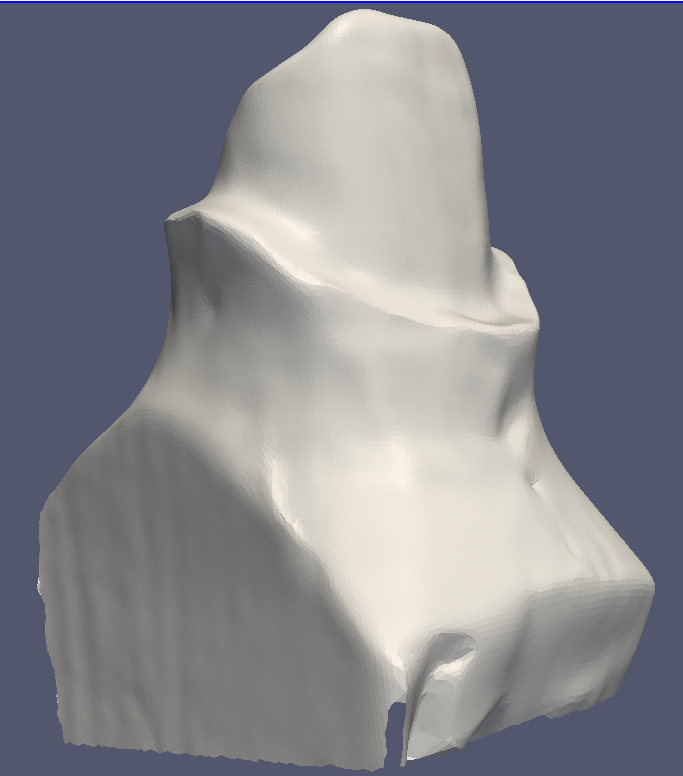
\includegraphics[width=2cm]{smooth_1}
	\centering
	\caption[res和expected的对比图示例]
	{res和expected的对比图示例.}
	\centering
\end{figure}

\section{分析}
准备从两个方向进行分析:
\subsection{平滑\&去噪}
\subsubsection{邻域的选取}
发现在使用Atos做光顺时,但选取小的过滤半径时,去噪声效果类似标准双边滤波的效果,而当选取比较大的过滤半径时,去噪效果优于标准双边滤波(Figure 2, Figure 3).\par
 因此猜测,要想得到理想的效果,应该动态地调整滤波邻域(半径,和点邻域还是边邻域),在整体比较平坦的地方使用顶点的1环邻域或更大的邻域.\par
如何来判断整体比较平滑?使用点的一环邻域,多做几次光顺之后,如果在边界面片附近,那么该面片使用边的一环邻域做光顺,否则就使用顶点的一环邻域或更大的邻域做光顺.(TODO)
\begin{figure}[H]
	\onecolumn
	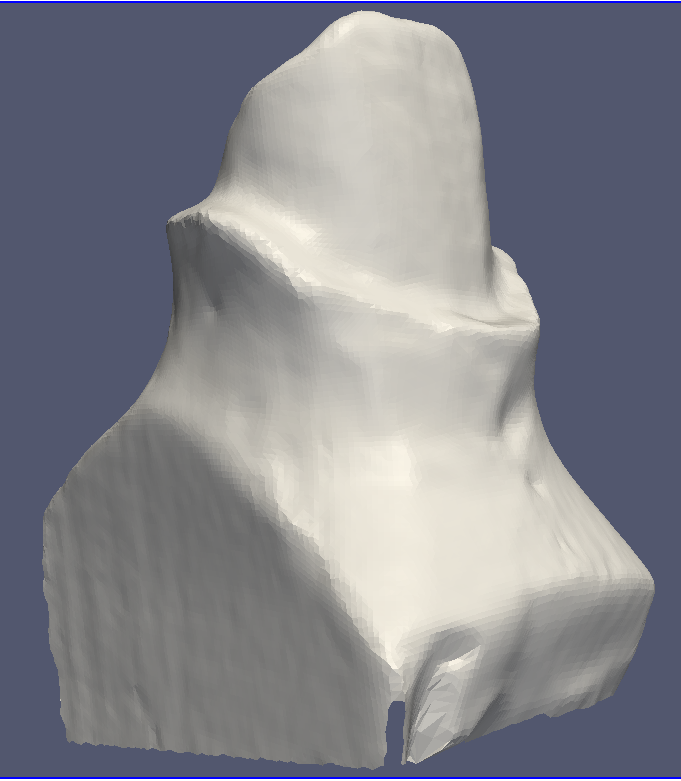
\includegraphics[width=6cm]{our_basic}
	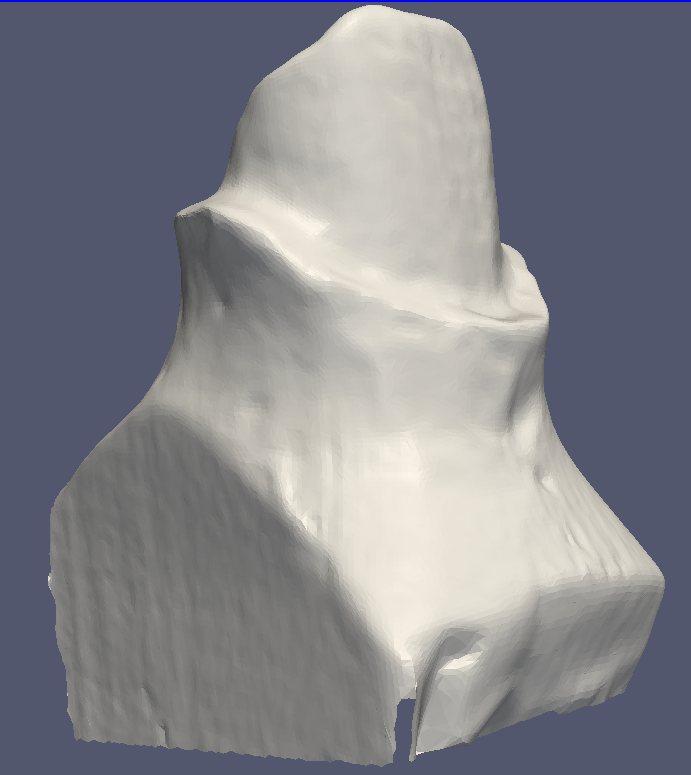
\includegraphics[width=6cm]{smooth_0}
	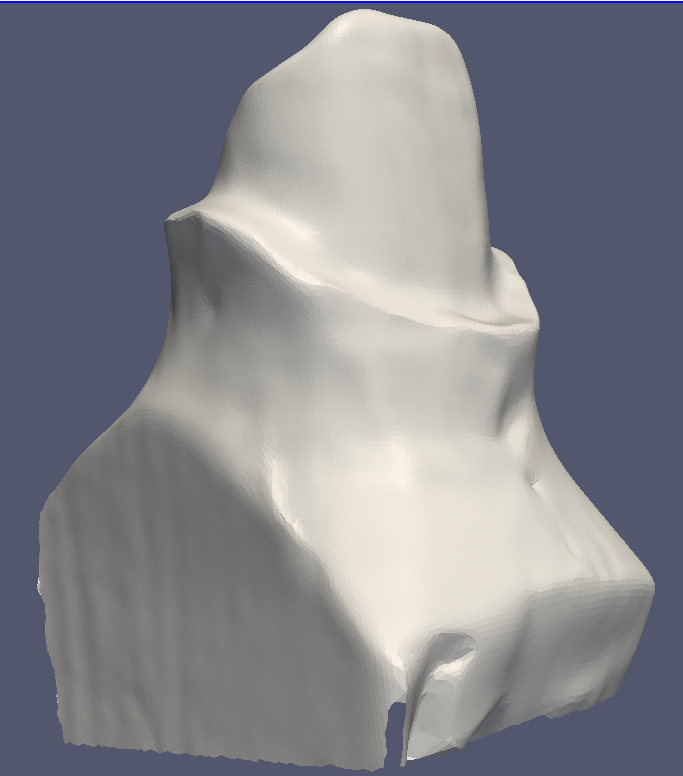
\includegraphics[width=6cm]{smooth_1}
	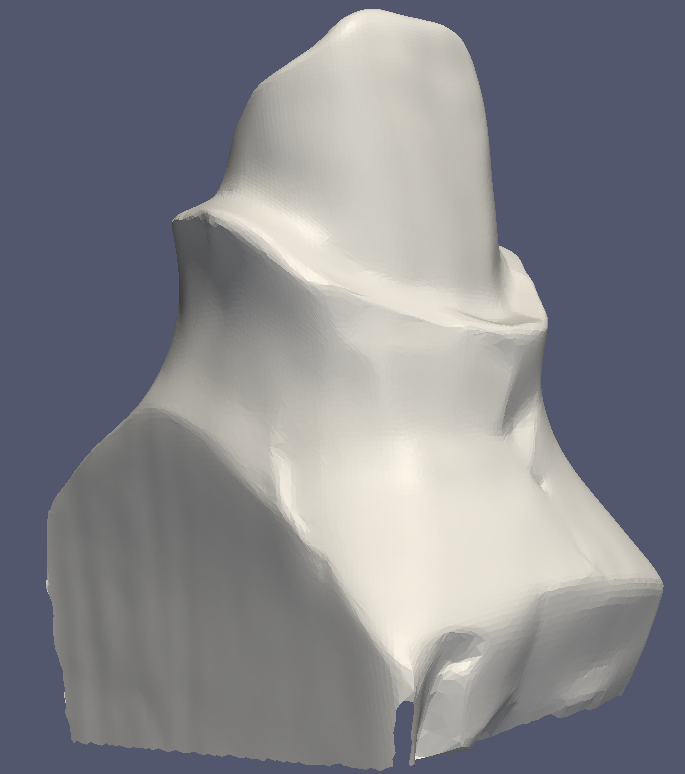
\includegraphics[width=6cm]{smooth_2}
	\caption[效果对比]
	{Atos不同程度光顺与标准双边滤波(3次迭代,边的一环邻域)效果对比,左上角为标准双边滤波效果,另外为geo inspect取不同滤波半径的结果,滤波半径依次扩大.}
	\centering
\end{figure}

\begin{figure}[H]
	\onecolumn
	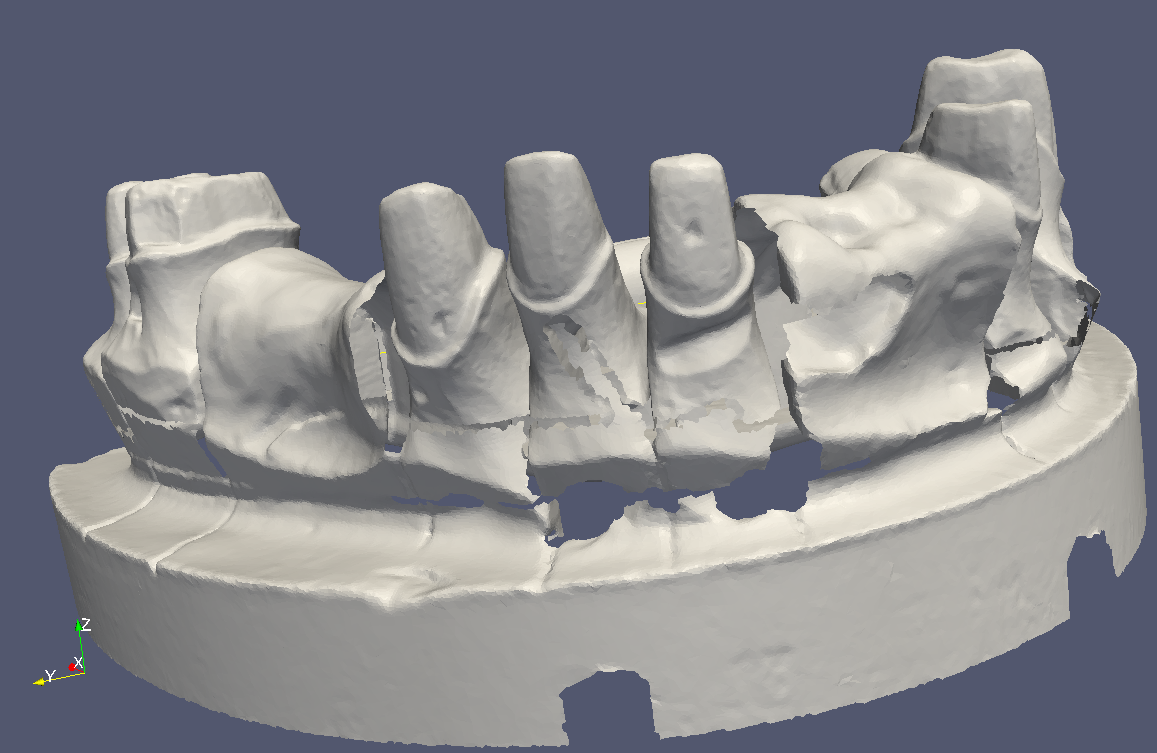
\includegraphics[width=6cm]{our_basic1}
	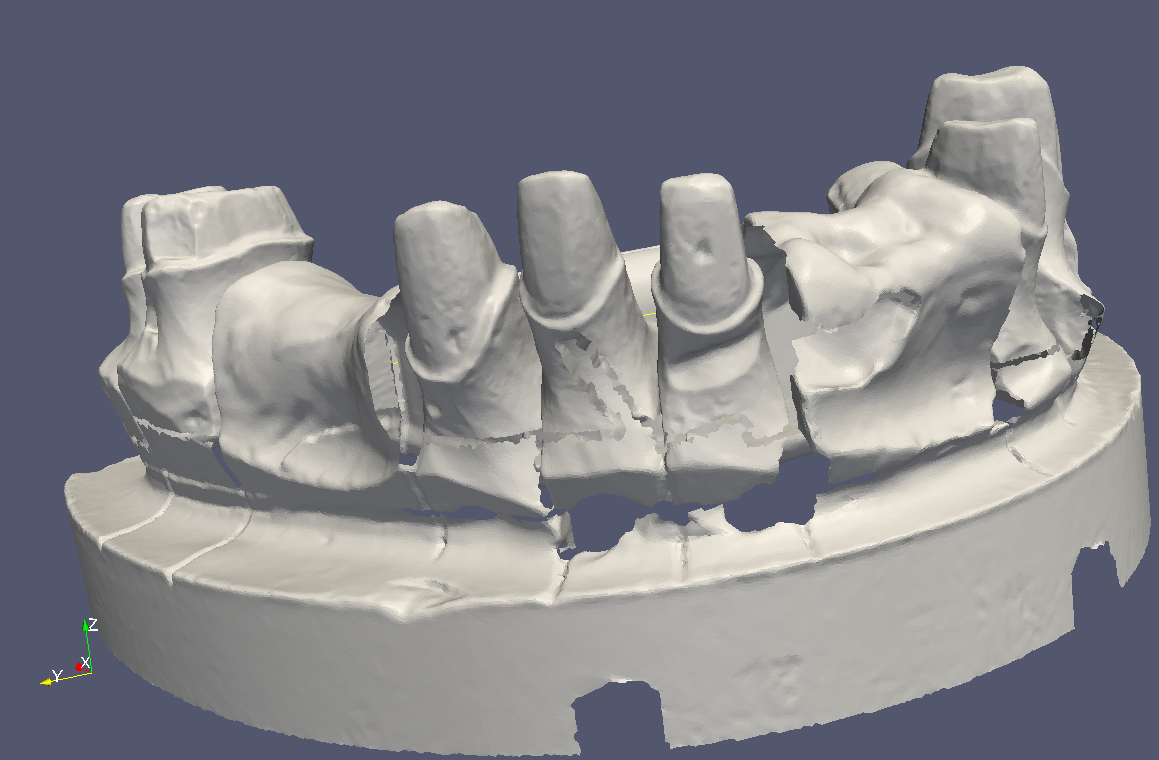
\includegraphics[width=6cm]{smooth1_0}
	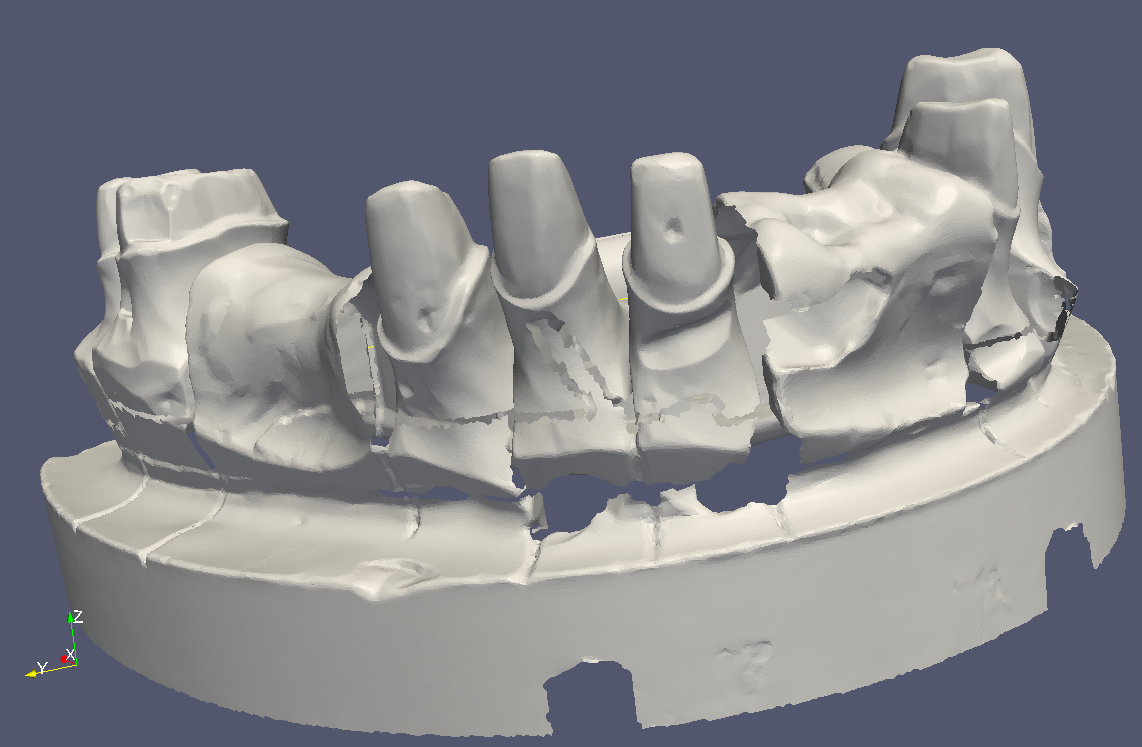
\includegraphics[width=6cm]{smooth1_1}
	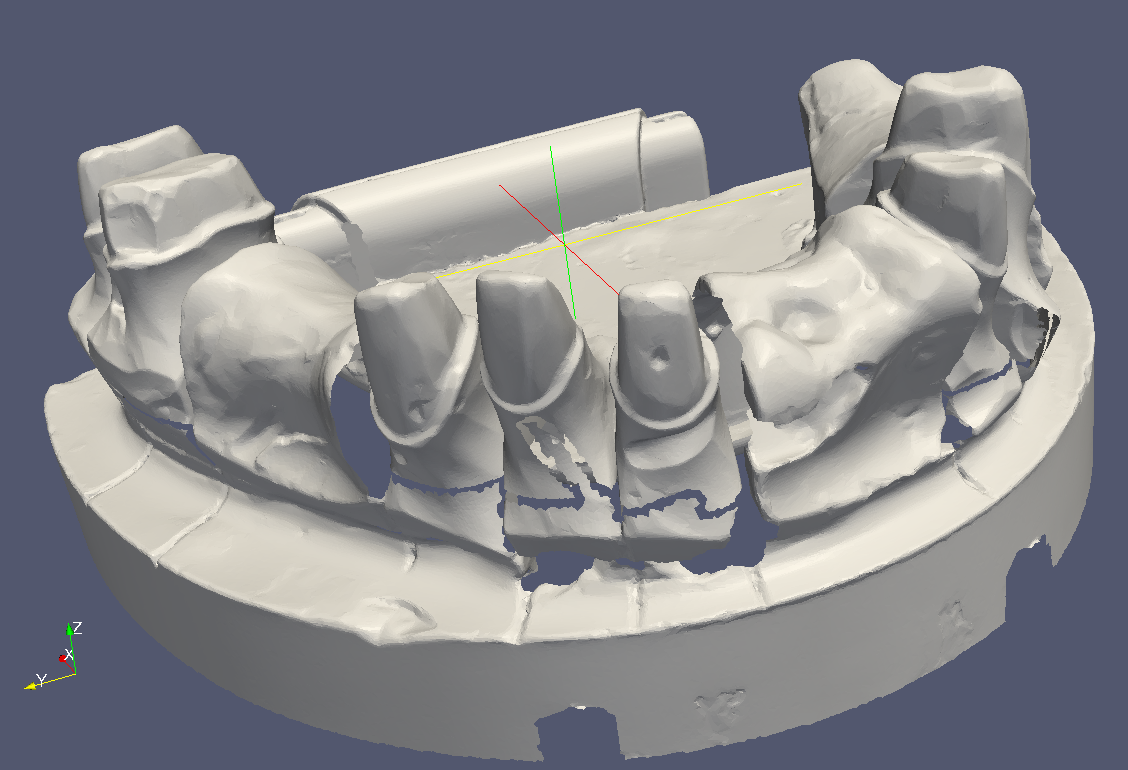
\includegraphics[width=6cm]{smooth1_2}
	\caption[效果对比]
	{Atos不同程度光顺与标准双边滤波(3次迭代,边的一环邻域)效果对比,左上角为标准双边滤波效果,另外为geo inspect取不同滤波半径的结果,滤波半径依次扩大}
	\centering
\end{figure}

\subsubsection{$\sigma_s$, $\sigma_c$的取值}
\subsection{细节锐化}
\end{document}
